%% Figure 1 of the manuscript, as a standalone source.
%% Lifted verbatim from the manuscript's tikzset block and tikzpicture on
%% 2026-09-11, when the manuscript switched to including the rendered image.
%% Redrawn on 2026-09-23: the dependence-channel box moved to Figure 2
%% (fig2_simulation.tex), the boxes have explicit equal heights, hyphenation is
%% off inside boxes, and every arrow is horizontal or vertical.
%% Build with: python3 build_fig1_framework.py <output_dir>
\documentclass[border=2pt]{standalone}
\usepackage{amsmath}
\usepackage{amssymb}
\usepackage{txfonts}
\usepackage{tikz}
\usetikzlibrary{arrows.meta,positioning}
\tikzset{
    box/.style={draw=black!70, rounded corners=1.5pt, align=left, inner sep=4pt,
        execute at begin node={\hyphenpenalty=10000\exhyphenpenalty=10000\relax}},
    inbox/.style={box, fill=black!3},
    stage/.style={box, fill=white},
    outbox/.style={box, fill=black!3},
    flow/.style={-{Latex[length=2.2mm,width=1.5mm]}, line width=0.65pt}
}
\begin{document}
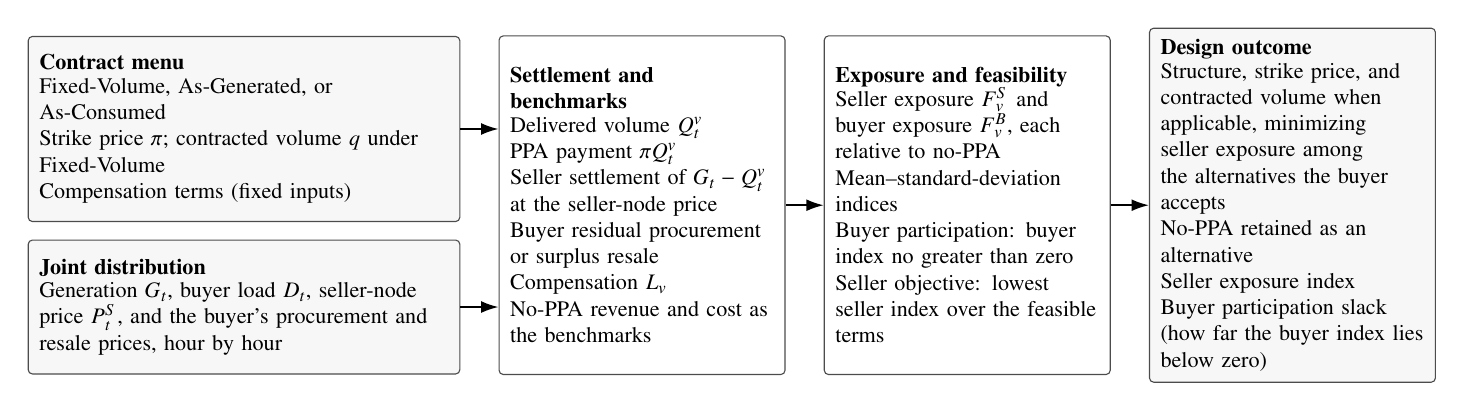
\begin{tikzpicture}[font=\footnotesize]

\node[inbox, text width=5.2cm, minimum height=2.35cm, anchor=north] (contract) at (0.0,2.15) {%
    \textbf{Contract menu}\\[-1pt]
    Fixed-Volume, As-Generated, or As-Consumed\\
    Strike price $\pi$; contracted volume $q$ under \mbox{Fixed-Volume}\\
    Compensation terms (fixed inputs)
};
\node[inbox, text width=5.2cm, minimum height=1.7cm, anchor=south] (joint) at (0.0,-2.15) {%
    \textbf{Joint distribution}\\[-1pt]
    Generation $G_t$, buyer load $D_t$, seller-node price $P_t^S$, and the buyer's procurement and resale prices, hour by hour
};
\node[stage, text width=3.35cm, minimum height=4.3cm] (settle) at (5.055,0) {%
    \textbf{Settlement and benchmarks}\\[-1pt]
    Delivered volume $Q_t^v$\\
    PPA payment $\pi Q_t^v$\\
    Seller settlement of $G_t-Q_t^v$ at the seller-node price\\
    Buyer residual procurement or surplus resale\\
    Compensation $L_v$\\
    No-PPA revenue and cost as the benchmarks
};
\node[stage, text width=3.35cm, minimum height=4.3cm] (expo) at (9.185,0) {%
    \textbf{Exposure and feasibility}\\[-1pt]
    Seller exposure $F_v^S$ and buyer exposure $F_v^B$, each relative to no-PPA\\
    Mean--standard-deviation indices\\
    Buyer participation: buyer index no greater than zero\\
    Seller objective: lowest seller index over the feasible terms
};
\node[outbox, text width=3.35cm, minimum height=4.3cm] (out) at (13.315,0) {%
    \textbf{Design outcome}\\[-1pt]
    Structure, strike price, and contracted volume when applicable, minimizing seller exposure among the alternatives the buyer accepts\\
    No-PPA retained as an alternative\\
    Seller exposure index\\
    Buyer participation slack (how far the buyer index lies below zero)
};
\draw[flow] (contract.east) -- (contract.east -| settle.west);
\draw[flow] (joint.east) -- (joint.east -| settle.west);
\draw[flow] (settle.east) -- (expo.west);
\draw[flow] (expo.east) -- (out.west);
\end{tikzpicture}
\end{document}
